\documentclass{article}
\usepackage[utf8]{inputenc}
\usepackage{amsmath}
\usepackage{amssymb}
\usepackage{graphicx}


\begin{document}
    \begin{titlepage}
        
        \centering
        {
\includegraphics[width=0.2\textwidth]{logo.png}\par}
        \vspace{1cm}
        {\bfseries\LARGE Universidad Nacional Autónoma de México \par}
        \vspace{1cm}
        {\scshape\Large Facultad de Estudios Superiores Acatlán \par}
        \vspace{3cm}
        {\scshape\Huge Ejercicio 2: Métodos de Bisección y Posición Falsa \par}
        \vspace{3cm}
        {\itshape\Large Materia: Métodos Numericos $1$ \par}
        \vfill
        {\Large Autor: Díaz Valdez Fidel Gilberto \par}
        {\Large Número de cuenta: 320324280 \par}
        \vfill
        {\Large Septiembre 2023 \par}
    \end{titlepage}


\section{Propósito}
Resolver un problema de aplicación empleando los métodos de acotamiento.

\section{Instrucciones}
Determinar el coeficiente de rozamiento \(c\), necesario para que un paracaidista de masa \(m = 71\) tenga una velocidad de \(42 \, \text{m/s}\), después de una caída libre de \(t = 13 \, \text{s}\). La aceleración de la gravedad es \(9.8 \, \text{m/s}^2\).

El problema se puede resolver determinando la raíz de la siguiente ecuación:
\[f(c) = gm\left(1 - e^{-\frac{ct}{m}}\right) - v\]

Donde:
\begin{itemize}
    \item \(t\) = tiempo
    \item \(v\) = velocidad
    \item \(m\) = masa
    \item \(g\) = gravedad
\end{itemize}

\section{Fórmula}
Primero partiremos de reemplazar los datos que conocemos en la fórmula para tener una idea más concreta de la función a graficar:
\[f(c) = (9.8)(71)\left(1 - e^{-\frac{c \cdot 13}{71}}\right) - 42\]

Ahora a partir de esta fórmula con los datos proporcionados graficamos para comprobar la existencia de una raíz.

\section{Gráfica}
La gráfica es la siguiente:
\\
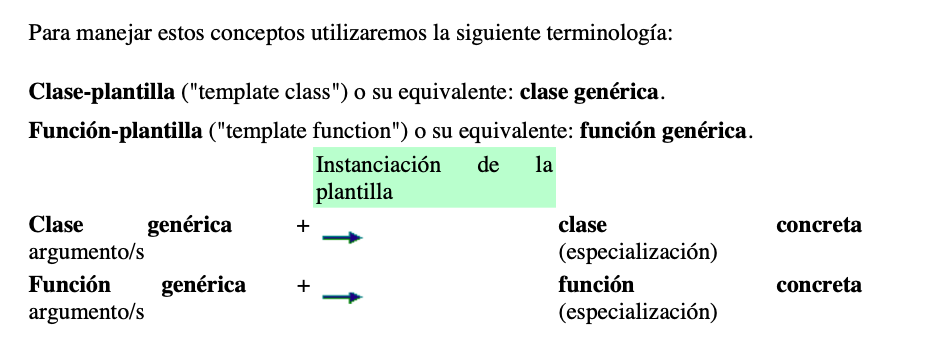
\includegraphics[scale=0.5]{Grafica.png}

\section{Elegir un intervalo de solución}
Analizando la gráfica más detenidamente se observa que su raíz puede estar entre el intervalo de [10, 20], por lo que lo tomaremos como intervalo inicial. Posterior a esto encontraremos su raíz por medio de dos métodos, serán los de Bisección y de Posición Falsa.

\section{Encontrar una raíz, con tolerancia \(0.00005\) en el error relativo y absoluto}

\subsection{Método de Bisección}
Usamos el intervalo que ya delimitamos contiene a la raíz y se continuará realizando en una hoja de cálculo los comandos y funciones pertinentes para llegar a la raíz.
\\
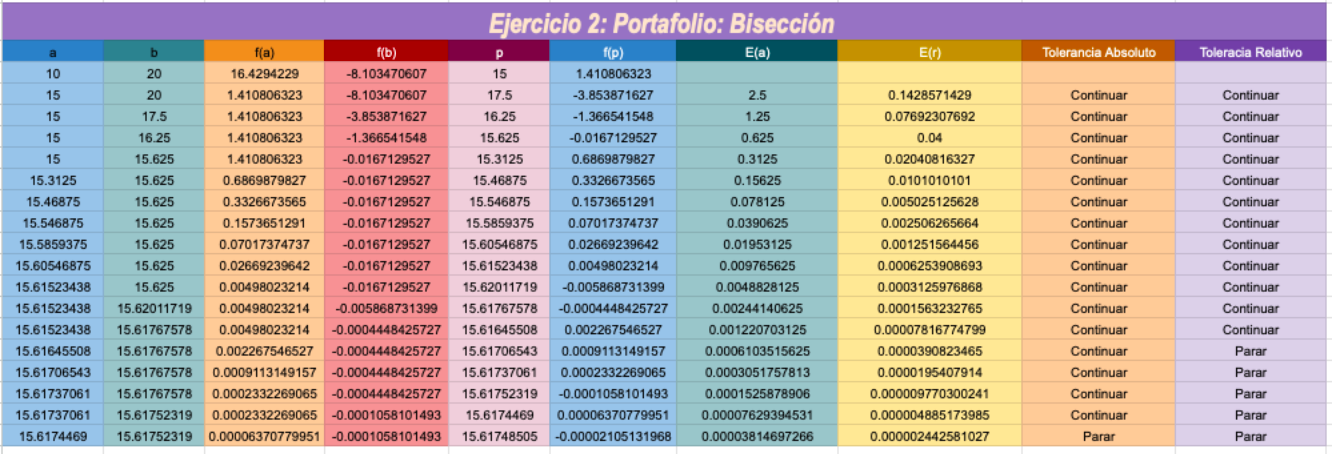
\includegraphics[scale=0.3]{Biseccion.png}

Primero se realiza la primera fila de acuerdo al intervalo escogido, la función y la evaluación de la misma a través de los extremos del intervalo [a, b], y calcular el punto medio de los intervalos para tomar ese punto \(p\) y evaluarlo en la función. De esta manera ya tenemos todos los datos necesarios para poder hacer uso de nuestra lógica e implementarla en el método.

Lo que se busca es encerrar a la raíz, por lo que los intervalos siempre, al ser evaluados, deben devolver valores de distinto signo, esto para asegurar que el intervalo contiene a la raíz. Nuestro intervalo [a, b] en específico ya devuelven imágenes de signo contrario al ser evaluadas en la función, lo que se debe hacer a continuación es:

\begin{itemize}
    \item Si el valor devuelto por \(p\) es del mismo signo que el devuelto por \(a\), \(p\) tomará el lugar de \(a\) y \(b\) será el mismo, pues así se tienen valores a evaluar que regresan imágenes de signo contrario.
    \item Similarmente se hará en el caso en el cual la imagen de \(p\) es del mismo signo de la imagen de \(b\), \(p\) pasará a tomar el valor de \(a\) y \(b\) quedará intacta.
\end{itemize}

Este proceso lógico continuará hasta llegar a la raíz al hacer el posible espacio donde esta se encontrará más pequeño, así se repetirá hasta llegar a ella o hasta lo que nos permita la tolerancia establecida.

Por último, será necesario el error absoluto que se calcula de la siguiente manera:
\[E_a = |x - x_n|\]

Donde \(x\) toma el valor exacto o el de la última \(p\) evaluada y \(x_n\) el de la aproximación o la \(p\) anterior a \(x\). Una vez calculado el error absoluto, haremos uso de la tolerancia que nos dieron. Si el error absoluto llega a ser menor de \(0.00005\), es momento de parar el proceso.

En el caso del error relativo, se aborda el mismo problema. Se calcula el error relativo de la siguiente manera:
\[E_r = \frac{|x - x_n|}{|x|}\]

A partir de este se compara con la tolerancia. Si el error es menor a la tolerancia, será momento de parar el proceso.

Como se puede observar, el proceso para en distintos momentos según la tolerancia al error utilizada.
\begin{itemize}
    \item Raíz con la tolerancia ligada al error absoluto: \(15.61748505\)
    \item Raíz con la tolerancia ligada al error relativo: \(15.61706543\)
\end{itemize}

\subsection{Método de Posición Falsa}
De igual manera se usará el mismo intervalo que con el método anterior, y se procederá configurando la hoja de cálculo que nos devuelva los datos necesarios.
\\
\begin{figure}[h]
    \raggedleft
    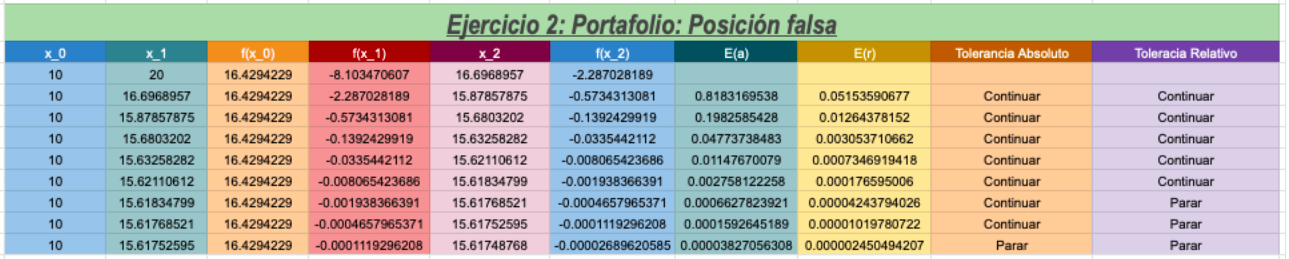
\includegraphics[scale=0.3]{Falsa.png}
    \end{figure}

Similar al método anterior, se parte del intervalo escogido \([x_0, x_1]\) y se realizan los cálculos y configuraciones con la hoja de cálculo para evaluar los puntos \(x_0\) y \(x_1\) en la función.

El gran cambio con este método es que no particionamos el intervalo a la mitad para tomar ese valor y evaluarlo, para en base a este hacer las demás condiciones e iteraciones hasta llegar a la raíz. Lo que se hace en este método es, a grandes rasgos, calcular por medio de conocimientos algebraicos y matemáticos a la \(x_2\) donde están cortando el eje de las \(x\) la recta tangente creada entre \(x_0\) y \(x_1\), en base a este cálculo y conociendo el valor de \(x_2\), se evalúa en la función y se analiza cómo continuar con la siguiente condición:
\begin{itemize}
    \item Si \(f(x_2)\) es de signo contrario que \(f(x_0)\), se cambiarán \(x_1 = x_2\), si esta condición es falsa, entonces \(x_0 = x_2\).
\end{itemize}
Como en este caso la condición sí se cumple, pues \(x_1\) tomará el valor de \(x_2\) para así empezar a acotar cada vez más a la raíz hasta que se llegue a ella, casi como si se tratara de un lazo que la va delimitando cada vez más y más. Pero ¿cómo funciona esto?
Pues al revisar la conclusión, sea el resultado falso o verdadero, esta condición está pensada para que sin importar el resultado se delimite a la raíz, ya que al las imágenes ser de distinto signo se asegura que la raíz se encuentra ahí, por lo que solo es necesario mover un valor y usar al otro como punto para trazar a la recta tangente que se acercará cada vez más hasta la raíz hasta alcanzarla, es como un barrido de la zona en donde se parte de un mismo punto, para a partir de este genrerar la recta con el otro punto y poco a poca acercarse mas a la raíz, casi como si se trazara un círculo.

Al completar la condición, lo único que continúa es seguir evaluando las \(x\) hasta llegar a una raíz o que nos detenga la tolerancia del error. En este caso nos detuvo la tolerancia primero, de igual manera ambas tolerancias nos detuvieron en momentos distintos:
\begin{itemize}
    \item La tolerancia al error absoluto nos da la raíz es: \(15.61748768\)
    \item La tolerancia al error relativo nos da la raíz es: \(15.61768521\)
\end{itemize}

\section{Conclusión}
Se observó que ambos métodos no llegan a la raíz, debido a que la tolerancia llega primero y por lo tanto nos obliga a parar, pero tambien considero que es importante tener en cuenta los intervalos que se tomaron para comenzar el mismo proceso.

No es lo mejor traer a la suerte en métodos numéricos ya que deberian ser efectivos dentro de un marco lógico y no causal, pero en este método sucede, pude haber escogido un intervalo que al biparticionarlo ya nos da el valor de la raíz debido a su cercania. En caso contrario con la poscición falsa la suerte se representa en la cercania que podriamos tener al escoger una $x$ a evaluar muy cercana a la raíz, esto provocaria que es menor el tramo que se debe recorrer a partir de esta para llegar a la raíz misma, la suerte radica en la capacidad de estar lo suficientemente cerca de la raíz desde un principio. 

En ambos casos la convergencia a la solción es lineal pero, como ya se puede observar en la magnitud de las gráficas, el método de bisección es mas tardado en acercarse a la raíz e incluso a la tolerancia de cualquier error, ya sea el absoluto o el relativo. Esto solo significa que este método se tarda mas en llegar a la raíz en si, también es importante denotar y observar que tanto la tolerancia al error absoluto como a la del relativo, en ambos métodos, se llegan a ellas en distintos puntos de la iteración. La razón por la que se me ocurre que sucede esto es por que en el error relativo se tiene en cuenta el hecho de que, al menos en este caso, se estan usando magnitudes distintas, cosa que no tiene en cuenta el error absoluto, de aqui parte la difernte tolerancia al error de cada una.

En conclusión el método de posición falsa es más eficaz que el de bisección, aunque no lo sea por mucho sigue siendolo, pero también es un poco más complicada y debe tener más una cierta comprensión y soltura algebraica además de consiencia matemática.
\end{document}
